\documentclass[11pt]{article}
\usepackage{graphicx}
\addtolength{\oddsidemargin}{-.875in}
	\addtolength{\evensidemargin}{-.875in}
	\addtolength{\textwidth}{1.75in}

	\addtolength{\topmargin}{-.875in}
	\addtolength{\textheight}{1.75in}
	
\usepackage{caption}
\usepackage{hyperref}
\usepackage{color}

\newcommand{\xvec}{\mbox{\bf x}}
\newcommand{\yvec}{\mbox{\bf y}}
\newcommand{\zvec}{\mbox{\bf z}}

\begin{document}

\title{\vspace{-0.25in} Robustness of Nonparametric Regression Using Kernelized Depth Function}
\author{}
\maketitle
\begin{flushleft}
\large
\vspace{0.1in}
\textbf{Abstract}
\vspace{0.1in}

We propose a robust method to reduce the impact of outliers on a given data set using kernelized spatial depth (see Chen et al. (2009)) and the Nadaraya-Watson estimator (see Nadaraya (1964) and Watson (1964)).

\vspace{0.1in}
\textbf{Introduction}
\vspace{0.1in}

The ordinary least square method to draw the best fit curve for linear data set fails under the presence of outliers.The least square method minimises the sum of squared distance between the observed response of data point and its predicted value.It shows significant deviations under corrupt data.
For polynomial functions Nadaraya-Watson estimator gives the best fit but it is also not reliable when the data set contains outliers. \\
Hence there is a need of robustness so that the useful information can be extracted from noisy data set and it founds applications in image processing,network security etc.

\vspace{0.1in}
\textbf{Step Towards Robustness-Median}
\vspace{0.1in}

We aim to minimise the weight of outliers as small as possible and to give  higher weights to the useful data. 
An outlier can be think of an observation which lies at an abnormal distance from other values in a random sample from a population. Generally, outliers are expected to appear more likely in outer layers with small depth values, than in inner layers with large depth values.But to identify the outlier in a data set we need some reference point.The reference point can be taken as mean or median but the mean is affected by the outlier and if the outlier goes to infinity then mean blows up.The better choice is to take median as the centre of observations and to decide the outliers with respect to median of dataset. \\
For any $\xvec \in \mathbf{R}$ , $\displaystyle{\vert \sum\limits_{i=1}^n S(\xvec_i-\xvec)\vert}$ gives the
  difference between the number of observations on the left and the right of $\xvec$ where S is the sign function and n is the number of observations.But for the median the number of observation on the right and left hand sides are equal hence sample median is any $\xvec \in \mathbf{R}$ that satisfies  $\displaystyle{\vert \sum\limits_{i=1}^n S(\xvec_i-\xvec)\vert}$=0.

For the higher dimensions the definition can be extended using Euclidean norm instead of absolute value. The multi-dimensional sample median for multi-dimensional data $\{\xvec_1,\ldots,\xvec_n\}\subset  \mathbf{R}^d$  is any $\xvec \in \mathbf{R}^d$ that satisfies
$$ \parallel \displaystyle{\sum\limits_{i=1}^n S(\xvec_i-\xvec)} \parallel =0,$$
where $\parallel \cdot \parallel$ is the Euclidean distance.Intutively median can be think of as a point for which the sum of unit vectors from that point to all other data points is zero.

\vspace{0.1in}
\textbf{Spatial Depth}
\vspace{0.1in}

The concept of spatial depth was first described by Vardi and Zhang.For a multivariate cumulative distribution function F on $ \mathbf{R}^d$ the spatial depth of a point  $\xvec \in \mathbf{R}^d$ with respect to the distribution F is defined as $$ D(x,\chi) =1-\displaystyle{ \parallel \int S(y-x)dF(y)\parallel} $$.

For an unknown cdf F,the spatial depth is unknown and it can be approximated by the sample spatial depth :$$ D(x,\chi) = 1-\frac{1}{\mid \chi \cup \{ \xvec \} \mid-1}  \displaystyle{\parallel \sum\limits_{y \in \chi} S(\yvec-\xvec) \parallel}. $$
Here, $\chi$ = $\{\xvec_1,\ldots,\xvec_n\}$ and $\mid \chi \cup \lbrace \xvec \rbrace \mid$ denotes the cardinality of union $\chi \cup \lbrace \xvec \rbrace$.\\ 

The range of $D(\xvec,\chi$) and $D(\xvec,F)$ is [0,1] . The depth value at the spatial median turns out to be 1 . Thus spatial median  have deepest depth . The spatial depth ranks the data points in terms of their depth value . The points lying in the outer part in the given data set have lower depth value as compared to the points lying near to the centre of the data point.So as we moves away from the deepest point to the outer points the depth value decreases from 1 to 0 . Thus we have the extremeness of the data points and this can be used to give weights or to classify the data points . Hence the outliers which disturb the data get a lower weight and the perturbation can be reduced.

 

\vspace{0.1in}
\textbf{Limitations of Spatial Depth functions}
\vspace{0.1in}

The spatial depth function works fine for the spherical symmetric distributions . But the spatial depth function may not capture the structure of a data cloud . A point lying in the outer parts in original data set may have higher depths as it happens in half-moon data . This is because the spatial depth function emphasizes only on the orientation of data set irrespective of the distance of a data point with respect to other data points . It depends only on the the sum of unit vectors from the point to observations.Hence it fails to put the fact in picture that extremity is significantly determined by the Euclidean distance.Hence to make the method robust by including appropriate metric functions .

\vspace{0.1in}
\textbf{Kernel}
\vspace{0.1in}

A positive definite kernel, k : $\mathbf{R}^d \times \mathbf{R}^d \rightarrow \mathbf{R} $ implicitly defines an embedding map $$ \phi: \xvec \in \mathbf{R}^d \longmapsto \phi(x) \in F$$ via an inner product in the feature space F, $$ k(\xvec,\yvec)=\langle \phi(x),\phi(y) \rangle , \xvec,\yvec \in \mathbf{R}^d$$.\\
Gaussian kernel  $K(\xvec,\yvec)=exp(-\Vert \xvec-\yvec \Vert^2/\sigma^2)$ determines the similarity measure between $\xvec$ and $\yvec$.

\vspace{0.5in}
\textbf{Kernelised Spatial Depth Function}
\vspace{0.1in}

Chen,Dang,Peng and Bart introduced Kernelised spatial depth function and made the spatial depth function applicable to a general dataset . They introduced the following:
$$ D_K(\xvec,\chi)= 1-\frac{1}{\mid \chi \cup \{ \xvec \} \mid-1} \left( \displaystyle{ \sum \limits_{\yvec, \zvec \in \chi} \frac{K(\xvec,\xvec)+K(\yvec,\zvec)-K(\xvec,\yvec)-K(\xvec,\zvec)}{\delta_K(\xvec,\yvec) \delta_K(\xvec,\zvec)}}\right)^{1/2},$$ 
where $K(\xvec,\yvec)=exp(-\Vert \xvec-\yvec \Vert^2/\sigma^2)$ and $\delta_K(\xvec,\yvec)=\sqrt{K(\xvec,\xvec)+K(\yvec,\yvec)-2K(\xvec,\yvec)}$. \\ \vspace{0.1in}
Note that $\displaystyle \frac{K(\xvec,\xvec)+K(\yvec,\zvec)-K(\xvec,\yvec)-K(\xvec,\zvec)}{\delta_K(\xvec,\yvec) \delta_K(\xvec,\zvec)}=0$ for $\xvec=\yvec$ or $\xvec=\zvec$.\\
\vspace{0.2in}
All the above calculations gives us the weight on each of the observation points . If the point lies far away from the data sets, then it has lower weight while if it lies closer to the data sets, then it has higher weight . 
The parameter $\sigma$ determines the size of the neighbourhood that is used to compute KSPD for an observation . When $\sigma$ is 0 then KSPD is constant, and when $\sigma$ is infinity KSPD goes to spatial depth .\\
\vspace{0.1in}
\textbf{Nonparametric Regression}
\vspace{0.1in}

If we have a random sample of bivariate data $(Y_1,X_1),\ldots,(Y_n,X_n)$ . The regression model is 
$$Y = m(X) + e,$$ 
where $m$ is an unknown function and $e$ is the random error . Nadaraya and Watson independently proposed the following estimator: 
$$m_{NW}(x)=\frac{\displaystyle{ \sum\limits_{i=1}^n K \left( \frac{X_i-x}{h} \right) Y_i}}{\displaystyle{ \sum\limits_{i=1}^n K \left( \frac{X_i-x}{h}\right )}},$$
where $K(u)=exp(-u^2)$ and $h>0$ is the smoothing parameter .\\
The method works well for the estimation of non-linear functions but when the outliers are present in the data set the predicted curve gets perturbed .\\
\vspace{0.1in}
\textbf{Robustness by Reweighting}
\vspace{0.1in}

We modify the Nadaraya-Watson estimator by applying weights to each of the data points as follows:
$$m_{1}(x)= \frac{\displaystyle{ \sum\limits_{i=1}^n D_K(\zvec_i,Z) K\left( \frac{X_i-x}{h} \right) Y_i}}{\displaystyle{ \sum\limits_{i=1}^n D_K(\zvec_i,Z) K\left( \frac{X_i-x}{h}\right )}},$$
where $\zvec_i=(y_i,x_i)$ for $i=1,\ldots,n$ and $Z$ is the collection of $n$ data points . 
This method is well-defined for more feature variables, i.e., multivariate $Y$ as well as multivariate $X$.

\vspace{0.9in}
\textbf{Simulations}
\vspace{0.1in}
\\
Consider 209 observations in the interval [0,1] with 9 outliers  and a polynomial mean function  $y=300(x^3-3x^4+3x^5-x^6)$ with normally distributed errors with variance $\sigma^2$=$0.3^2$ and mean 0 where
$\xvec$ ranges from 0 to 1 in arithmetic progression and consist of 200 observations.



  
We computed  the kernelised depth function and then the weighted and general Nadaraya-Watson Estimator   for each data point.This is done by varying the parameters $\sigma$ and smoothing parameter h to get the robust fit .\\
\vspace{0.1in}
 For this we executed our algorithm on h values ranging from 0.01 to 0.1 in a arithmetic series with a common difference of 0.01 . Another set of h values range from 0.2 to 5 in a arithmetic progression with a common difference of 0.533.

\vspace{0.1in}



 $\sigma$ values range from $2^{-8}$ to $2 ^{11}$ in a geometric progression with common ratio of 2.




\vspace{0.1in}

\begin{figure}[ht]
\begin{center}
% \vspace{-0.5in} 
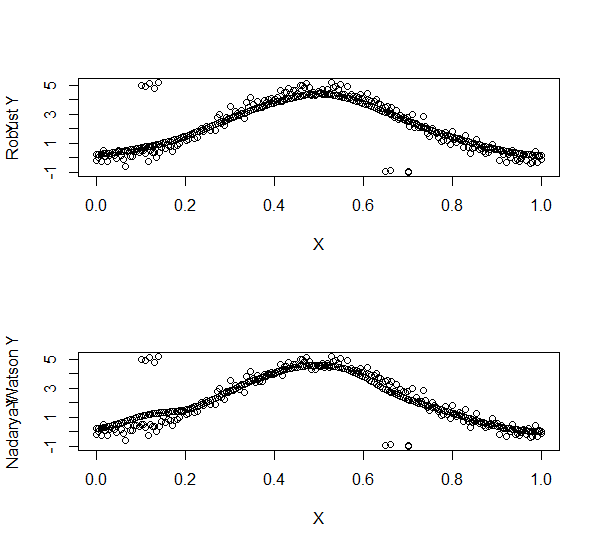
\includegraphics[scale=0.8]{Rplot}

\end{center}
\end{figure}

Then we find out the Euclidean distance between the underlying polynomial function and the function obtained by our proposed method for each of the above h and sigma values and we obtained the minimum Robust distance of  0.03465705 corresponding to h=0.01 and $\sigma$ =2048 .

\vspace{0.1in}

Simultaneously we find out the Euclidean distance between the underlying polynomial function and the function obtained by the Nadaraya and Watson Estimator for each of the above h and sigma values and we obtained the minimum Nadaraya -Watson distance of  0.1509096 corresponding to h=0.05 and $\sigma$ =0.00390625 .


 
 \vspace{0.1in}
 \textbf{Multidimensional Simulations}
\vspace{0.1in}

Consider 227 observations and function  $y=-8000(e^{v}e^{10u})$  consisting of 27 outliers  and  normally distributed errors having variance $\sigma^2$=$100$ and mean 0  where  $u \in$  [0,1] and v $\in$ [10,11] ,each containing 200 points in arithmetic progression in the above range.\\
 

\vspace{0.1in}


For this we executed our algorithm on h values ranging from 0.01 to 0.1 in a arithmetic series with a common difference of 0.01 . Another set of h values range from 0.2 to 5 in a arithmetic progression with a common difference of 0.533.
\vspace{0.1in}
and following $\sigma$ values 


 [1,] 89558784586
 [2,]       97896
 [3,]         500
 [4,]        6000
 [5,]         789
 [6,]       12345
 [7,]      658967
 [8,]       58586
 [9,]          11



\begin{figure}[ht]
\begin{center}
% \vspace{-0.5in} 
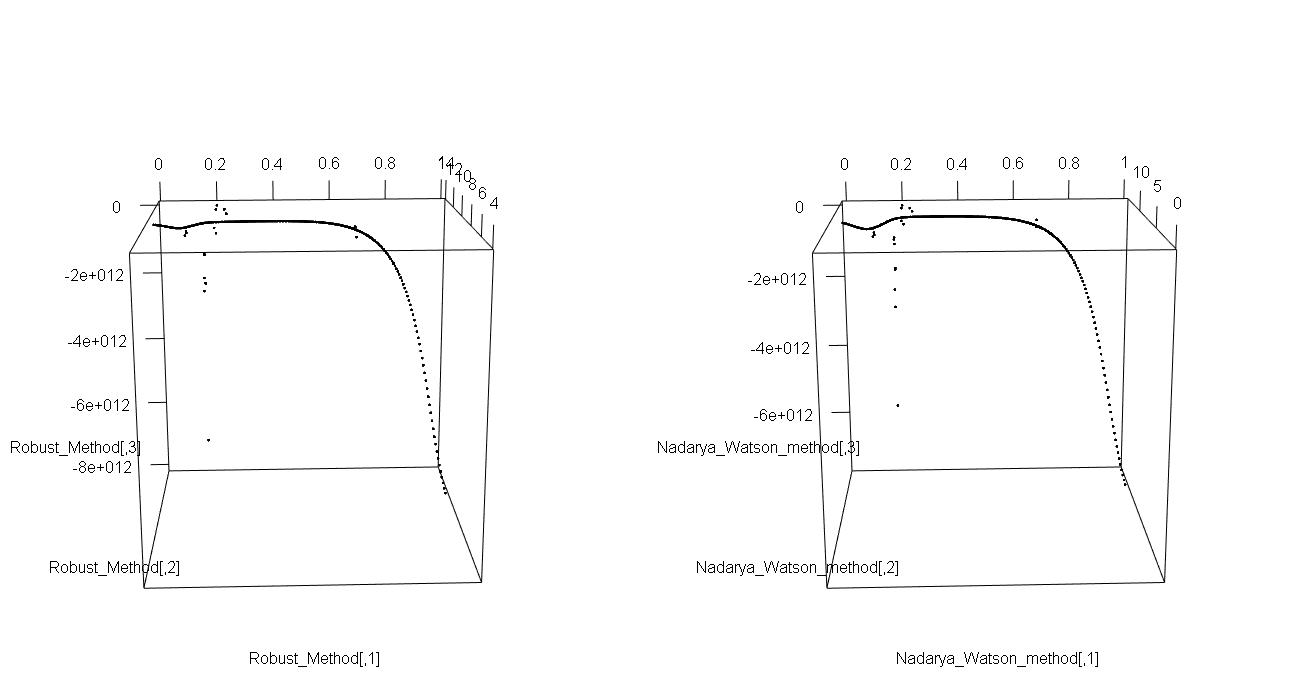
\includegraphics[scale=0.4]{4}

\end{center}
\end{figure}

 Then we find out the Euclidean distance between the underlying  function and the function obtained by our proposed method for each of the above h and sigma values and we obtained the minimum Robust distance of  1.951308e+23  corresponding to h=0.05 and $\sigma$ =89558784586.
 
 Simultaneously we find out the Euclidean distance between the underlying function and the function obtained by the Nadaraya and Watson Estimator for each of the above h and sigma values and we obtained the minimum Nadaraya -Watson distance of  2.635321e+23 corresponding to h=0.06  and $\sigma$ =89558784586 .
 
 \vspace{0.42in}
\textbf{Future Work}
\vspace{0.1in}
\begin{itemize}
 \item  We need to devise a robust and computationally efficient version of the general leave-one-out cross
validation  defined by 
$$ CV=\frac{1}{n}\displaystyle{\sum\limits_{i=1}^n(Y_i-m_{(-i)}(x_i)})^2$$
where $m_{(-i)}(x_i)$
is the estimator obtained by omitting the $i^{th}$
pair $(X_i
, Y_i)$.This will lead to a better prediction of the smoothing parameter.

 \item We also want to investigate the performance of the $0-1$ weight function by classifying the data set on the basis of calculated Kernalised spatial depth with reference to a particular threshold.
\end{itemize}






\vspace{0.2in}
\textbf{References}
\vspace{0.1in}

\small

Chen, Y., Dang, X., Peng, H., and Bart, H. L. (2009) Outlier detection with the kernelized spatial depth function. IEEE Transactions on Pattern Analysis and Machine Intelligence, 31(2), 288-305.
\vspace{0.05in}

% De Brabanter, K., De Brabanter, J., Suykens, J. A., Vandewalle, J., and De Moor, B. (2012) Robustness of kernel based regression: Influence and weight functions. In Neural Networks (IJCNN), The 2012 International Joint Conference on (pp. 1-8). IEEE.
% \vspace{0.05in}

Nadaraya, E. A. (1964) On estimating regression. Theory of Probability and Its Applications, 9(1), 141-142.
\vspace{0.05in}

Serfling, R. (2002) A depth function and a scale curve based on spatial quantiles. In Statistical Data Analysis Based on the L1-Norm and Related Methods (pp. 25-38). Birkhäuser Basel.
\vspace{0.05in}

Vardi, Y., and Zhang, C. H. (2000). The multivariate L1-median and associated data depth. Proceedings of the National Academy of Sciences, 97(4), 1423-1426.
\vspace{0.05in}

Watson, G. S. (1964) Smooth regression analysis. Sankhya: The Indian Journal of Statistics (Series A), 26(4), 359-372.














\end{flushleft}


\end{document}
